% 
% chapter4.tex
% ThesisISEL
% 
% Created by Serge Lage on 2019/07/30.
%
% ================
% = Blue Box =
% ================
\chapter{Standalone Fishery Analysis}
\label{cha:standalone_fishery_analysis}
This chapter explains the approach used to reach the first goal of this work. It describes an application that implements the work done in this chapter with respect to its functionality, architecture, implementation details and usage. 


The first objective is to develop a locally implemented tool that registers whether the vessel is engaged in fishing, and if so, whether the fishing area is new or is habitual. This solution must be implemented by the vessel. Therefore each vessel will only have access to its data. That is, each vessel only will know it is one data. This data consists of VMS data described in Section 3.1 VMS Records.

The solution developed to meet this objective consists of a machine learning application to analyze data in real-time, to determine whether the vessel is fishing, and if so, whether it is fishing in its fishing zone or a new location.
The fact that this analysis is done by vessel allows avoiding bias in results each vessel has a different power, size and its suitable for specific fishing activity.\\
This solution could be implemented and used as a library by the MONICAP system shown in Figure \ref{fig:monicap} .\cite{WEBSITE:MonicapXsealence}.

\begin{figure}[H]
\centering
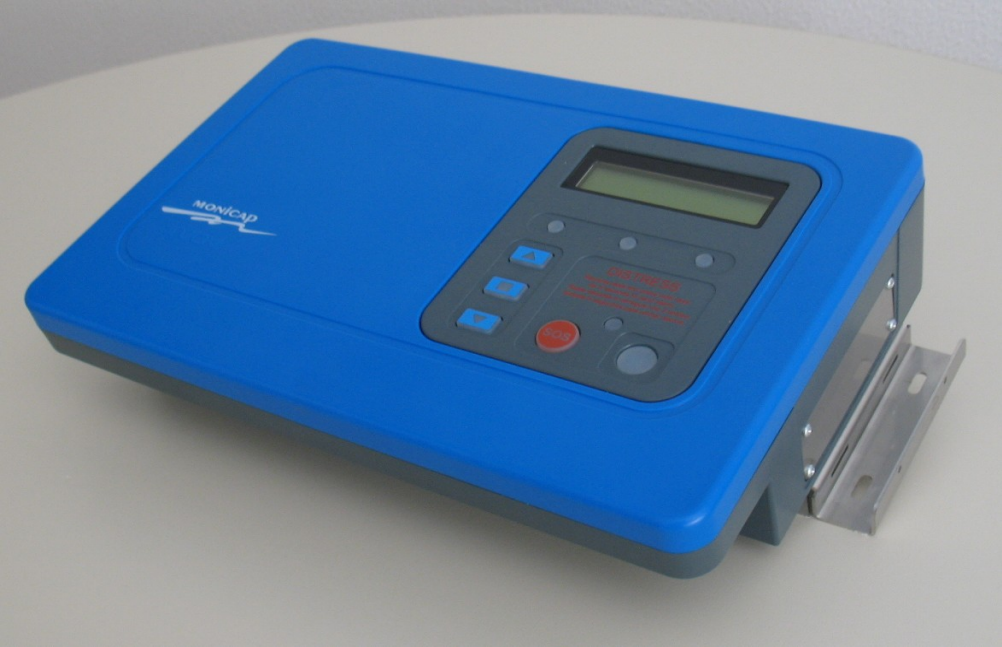
\includegraphics[width=0.8\linewidth]{Chapters/img/equipamento_monicap.png}
\caption{MONICAP Blue Box.}
\label{fig:monicap}
\end{figure}

As MONICAP systems are installed on ships, they can, in real-time, send alerts to the authorities whenever an abnormal change is detected concerning the standard.


\section{Fishing Velocity Patterns} % (fold)
\label{sub:fishing_velocity_patterns}

To know whether a vessel is fishing, we can use it is velocity patterns, given that the speed of the vessel differs where it is traveling or when it is fishing. We can verify this fact in the histogram shown in Figure \ref{fig:histogram_vessel2}, corresponding to a vessel velocity.

In Figure \ref{fig:histogram_vessel2}, the histogram allows us to recognize two different velocity patterns, identified by two distinct distributions. They are visible when we graphically represent the velocity's data of each of the vessels. The distribution characterized by lower average speeds corresponds to fishing activity, and the other speed distribution corresponds to the movement of the vessel between the port and the fishing sites.\\
So, it is needed to isolate the first distribution's range to be able to classify the upcoming future velocity's as fishing associated or not.
\begin{figure}[H]
\centering
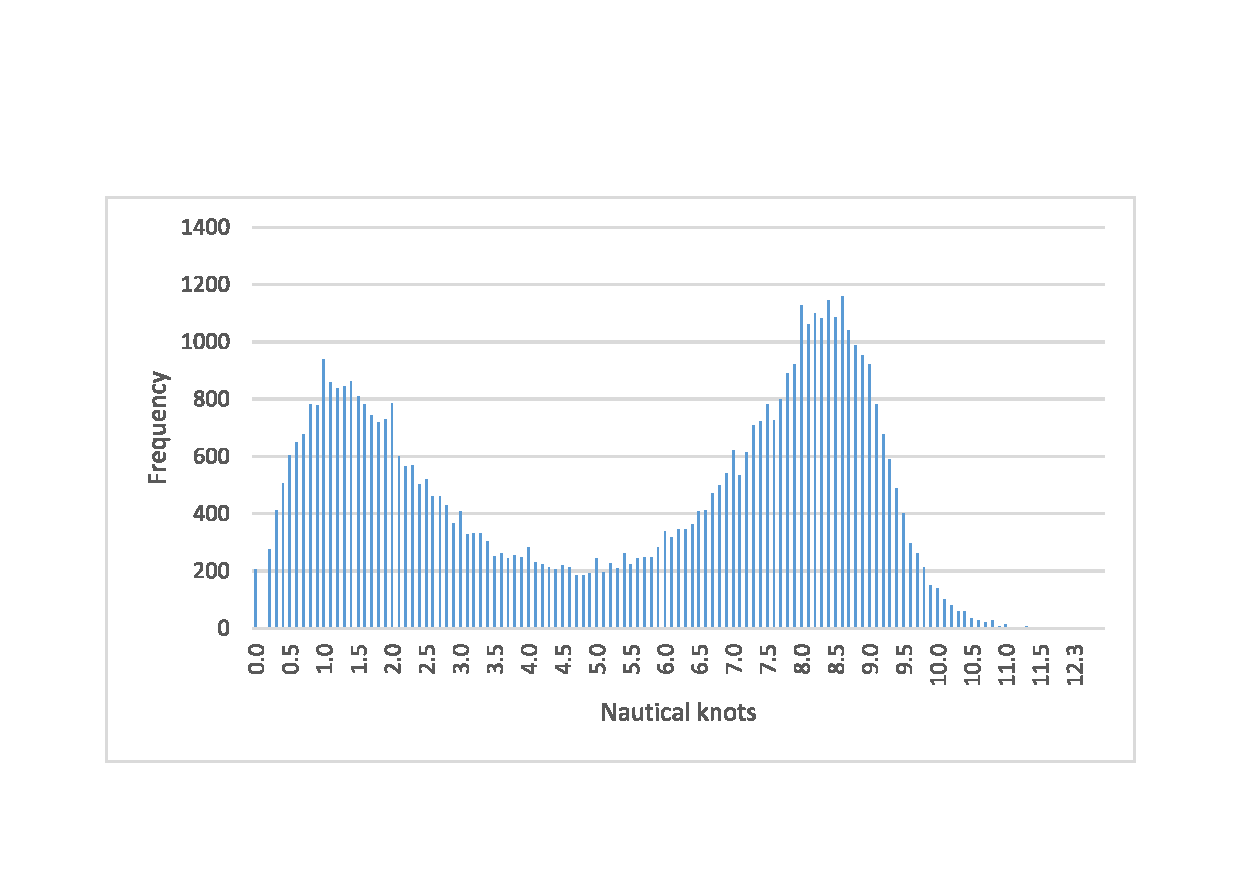
\includegraphics[trim=0 50 0 50, width=0.8\linewidth]{Chapters/img/hist_vessel2.pdf}
\caption{SOG Histogram vessel 2.}
\label{fig:histogram_vessel2}
\end{figure}


For the propose of isolating the first distribution was considered three optional procedures:
\begin{itemize}
\item \textbf{Standard deviation:}
This solution assumes that the velocity distribution is normal. Using the distribution of the fishing velocity, we find the fishing velocity with more occurrences and with the standard deviation, we can choose a distance from the mean. So we can get the minimum population desired (explained by Chebyshev's inequality \cite{Chebyshevinequality}) to be within the fishing range. \\
Pros and cons: This solution is simple and fast to implement, but we are not working with a normal distribution.

\item \textbf{Kernel Density Estimation:}
Kernel Density Estimation method estimates the probability density function by imposing a model function on every data point and then adding them together. The function applied to each data point is called a kernel function \cite{KernelDensityEstimation}.
Pros and cons: This solution gives us a way to configure the threshold for the fishing distribution limits. This solution will not work because the density distribution for the velocity will differ from vessel to vessel. 

\item \textbf{Filter:}
Use a Hill-Climbing algorithm\cite{Kvasnicka1995HillCW}. This algorithm is a local optimization algorithm which provides a direct search. The Stochastic Hill-Climbing algorithm works supported in an iterate process of randomly selecting a neighbor for a candidate solution. The acceptance of the solution is conditioned by a criterion of improvement concerning the previous solution. With this algorithm, find the fist maximum and then find the next minimum.
Then remove all the velocity occurrences that happen less than 10 \% of the maximum occurrence and isolating the occurrences that are fallowed. We can retrieve a clean distribution of the fishery speed of that vessel. With this, we can use the first and last values to classify the new inputs. 
Pros and cons: Solution that is independent of fishing type distribution. Needs to organize the velocity data for the Hill-Climbing algorithm. Create a version that finds the local maximum and then finds the next minimum.
\end{itemize}

The selected procedure can be described in two steps: it starts by using the method based on the \textbf{Filter} to isolate the fishery speed from the remain. Then the Kernel distribution method was applied.
\begin{enumerate}
\item \textbf{Filter:} In the first step, it retrieves all velocity data from the database to create a histogram like it is shown in Figure \ref{fig:histogram_vessel2}. In the next step, it uses the hill-climbing algorithm to get the minimum and the maximum value of the first distribution. 
The implementation used was altered in a way that when the algorithm converges to the maximum, it will continue to find the limit of the distribution.
To obtain this solution, the algorithm searches for the first local maximum that does not have a higher value in the following three points. In this way, we can find the maximum value of the fishing speed range. \\
To find the end of the fishing speed range, the algorithm continues to sweep the histogram until the next three points are not lower than the current point.
Velocity 0 is removed because we do not want to consider when the vessel is completely stopped. 
This way, we can end up with a histogram of the intended distribution, as we can observe in Figure \ref{fig:sog_hill_climbing}.

\begin{figure}[H]
\centering
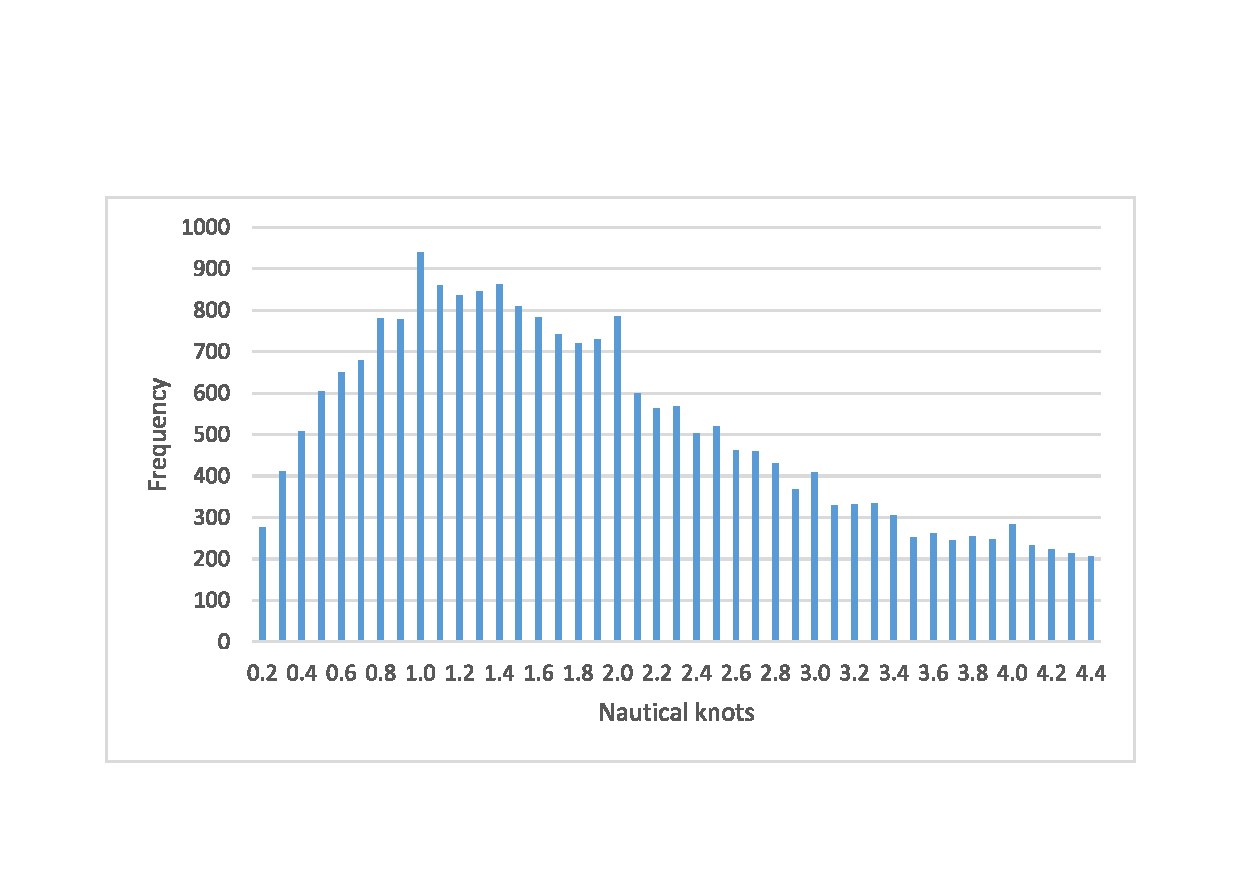
\includegraphics[trim=0 50 0 50,width=0.8\linewidth]{Chapters/img/sog_hill_climbing.pdf}
\caption{Velocity distribution of vessel 2 after the application to the Hill Climbing algorithm}
\label{fig:sog_hill_climbing}
\end{figure}


\item \textbf{Kernel:} It was applied a kernel distribution method in the filtered histogram to have the distribution represented in orange on \ref{fig:hist_kernel}. Then it was created a dictionary with the velocities and the cumulative percentage of velocity. This way, we end up with a histogram like the one represented in Figure \ref{fig:hist_comulative}. 
Then a range across quantiles is defined for some probability. As in the estimation of confidence intervals, a confidence level is also defined here, which will be associated with the two-speed limits that correspond to the fishing activity.
\end{enumerate} 

\begin{figure}[H]
\centering
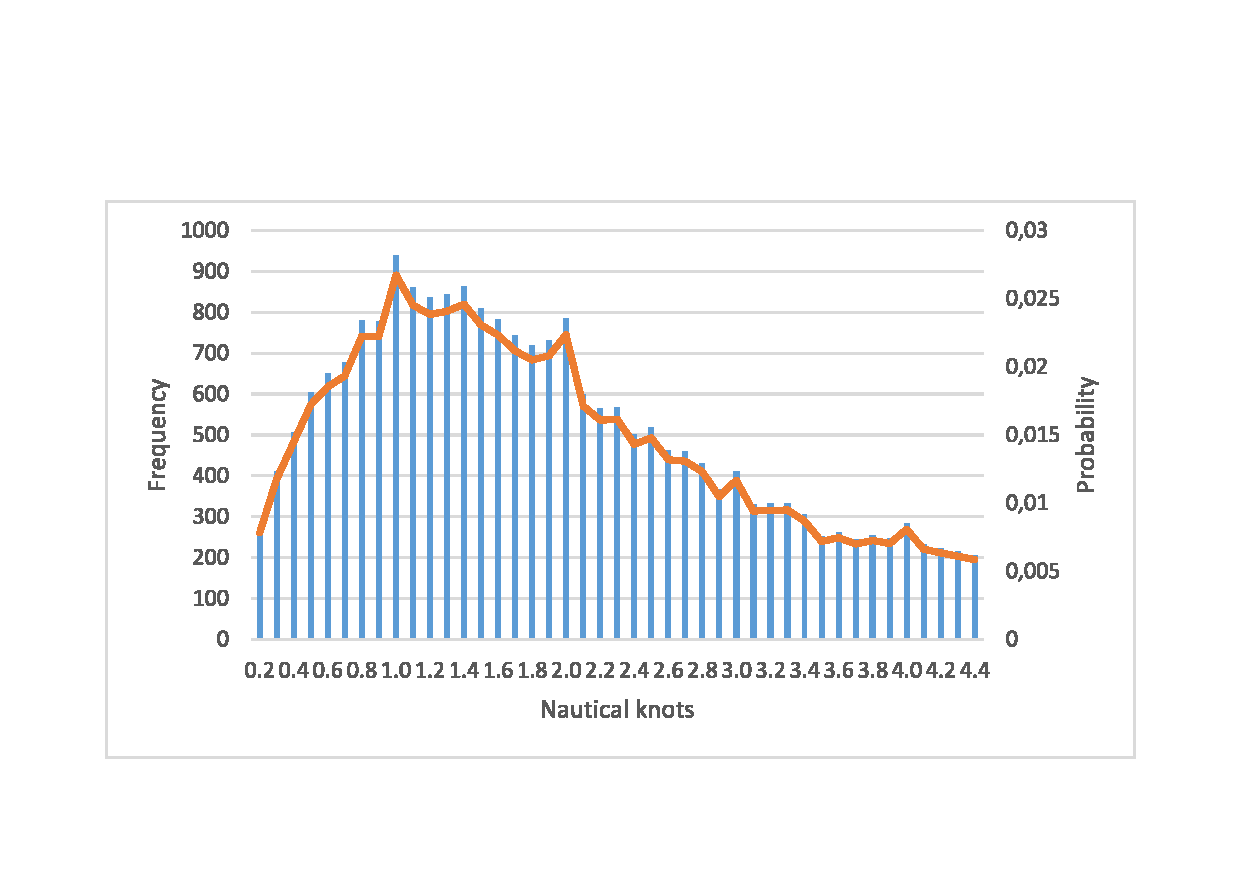
\includegraphics[trim=0 50 0 50,width=0.8\linewidth]{Chapters/img/hist_kernel.pdf}
\caption{Kernel density distribution filtered data}
\label{fig:hist_kernel}
\end{figure}


Now we can compare the new data with the established limits. If the new data is within limits, we classify as fishing, and if not, we classify as not fishing.

\begin{figure}[H]
\centering
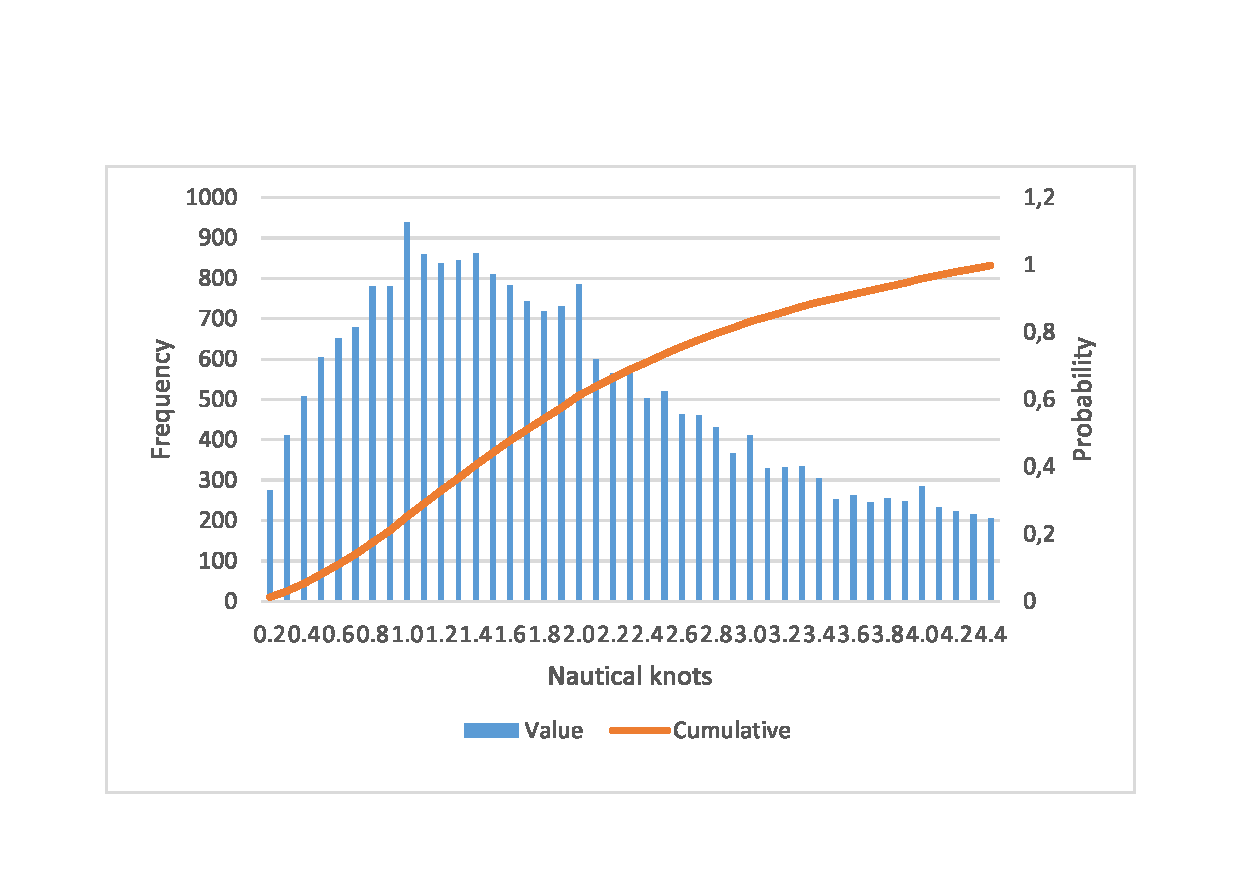
\includegraphics[trim=0 50 0 50,width=0.8\linewidth]{Chapters/img/hist_comulative.pdf}
\caption{Filtred histogram with cumulative kernel distribution}
\label{fig:hist_comulative}
\end{figure}

Appendix B has presented the functionality of this algorithm, step by step. 

% section fishing_velocity_patterns (end)


\section{Fishing Spots} % (fold)
\label{sub:fishing_spots}

To discover whether the
the vessel is fishing in its fishing zone, or a new location, the history of GPS locations by vessel was used.
Fishing in a new zone may mean that the vessel has changed its type of fishing or is engaging in an activity that is not licensed.


\begin{figure}[H]
\centering
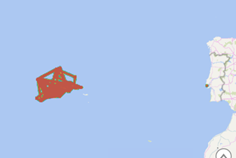
\includegraphics[width=0.8\linewidth]{Chapters/img/gps_vessel2.png}
\caption{Vessel 2 GPS points}
\label{fig:gps_vessel2}
\end{figure}

In Figure \ref{fig:gps_vessel2}, we can see the GPS points of a vessel. Using methods based on clustering, it is possible to identify several areas by a vessel that are the standard fishing zones of the vessel. When the vessel is outside that zone, a flag should occur.

Using the fishing velocity range encountered in the previous point, we get the GPS points of the vessel within that range, so we can work only with the positions where the vessel was fishing. The next step is to use a clustering algorithm to define the fishing areas so that we can compare it with the new GPS points. 

For this purpose, several data mining algorithms were performed to choose the best results:

\begin{itemize}
\item \textbf{K-Means:}
K-means clustering algorithm \cite{HitchcockKmeans} is a method of cluster analysis which aims the partition of n observations into k clusters in which each observation belongs to the cluster with the nearest mean. This results in a partitioning of the data space. K-means (Macqueen, 1967) is one of the simplest unsupervised learning algorithms that solve the well-known clustering problem. The procedure follows a simple and easy way to classify a given data set through a certain number of clusters (assume k clusters) fixed a priori. The main idea is to define k centroids, one for each cluster. These centroids should be placed cunningly because of different location causes a different result. So, the better choice is to place them as much as possible, far away from each other. The next step is to take each point belonging to a given data set and associate it to the nearest centroid. When no point is pending, the first step is completed, and an early group is done. At this point, we need to recalculate k new centroids as bar centers of the clusters resulting from the previous step. After we have these k new centroids, a new binding must be done between the same data set points and the nearest new centroid. A loop has been generated. As a result of this loop, we may notice that the k centroids change their location step by step until no more changes are done.

\item \textbf{Density Based Cluster:}
Density-based clustering algorithms \cite{WekaCC} try to find clusters based on the estimation of the density of data points in a region.
It can find arbitrarily shaped clusters and handles noises and yet is a one-scan algorithm that needs to examine the raw data only once. In density-based clustering algorithms, dense areas of objects in the data space are considered as clusters, which are segregated by low-density area (noise). The basic idea of density-based clustering is that clusters are dense regions in the data space, separated by regions of lower object density \cite{WEKATalankiDensity}.
The key idea of density-based clustering is that for each instance of a cluster, the neighborhood of a given radius (Eps) must contain at least a minimum number of instances (Min Pts).

\item \textbf{DBSCAN:}
DBSCAN (for density-based spatial clustering of applications with noise) is a data clustering algorithm proposed by Martin Ester, Hans-Peter Kriegel, Jorge Sander and Xiaowei Xu in 1996 It is a density-based clustering algorithm because it finds several clusters starting from the estimated density distribution of corresponding nodes. DBSCAN \cite{Kisilevich2010PDBSCANAD} is one of the most common clustering algorithms and most cited in the scientific literature.
\end{itemize}

After some tests, it was decided that Density-Based Cluster is the best approach for this case. It was excluded DBSCAN, because as we can observe in \ref{table:mill_per_moodle}, this model needs much processing power to estimate the clusters. These values were retrieved using a computer with an Intel i5 (2.5 GHz) and 8 GB of RAM. Considering that the Blue Box as a lot less processing power, it was decided that this model is not a good solution for this problem.
\\

\begin {table}[H]
\begin{center}
\begin{tabular}{c|c|c|c}
& \textbf{K-Means} & \textbf{Density Based Cluster} & \textbf{DBSCAN} \\
\hline
Initializing & 862 & 923 & 25848 \\

New data & 25 & 45 & 35 
\label{table:mill_per_moodle}
\end{tabular}
\caption {Milliseconds per model}
\end{center}
\end {table}

The choice between K-Means and Density-Based Cluster algorithms was based on the fact that Density-Based Cluster represents a great advantage because it estimates the probability of the new GPS point belonging to a cluster-based in the cluster probabilistic distribution. This way, the user can choose the most suitable configuration. The resulting clusters themselves are equal when K-Means or Density-Based Cluster were applied since Density-Based Cluster uses K-Means to define the centroids, so they only differ by adding a layer to define the area of density per cluster.
\\
To decide the number of clusters to use, it was used the elbow method \cite{Kodinariya2013ReviewOD}, for the within-cluster sum of squares, as could be seen in Figure \ref{fig:elbow_method}. The within means the distance the vectors in each cluster are from their respected centroid. The goal is to get this number as small as possible. One approach to handling such an objective is to run the K-means clustering multiple times, raising the number of the clusters each time. Then it is possible to compare the withinss each time, stopping when the rate of improvement drops off. The better case corresponds to find a low withinss while still keeping the number of clusters low.\\
The elbow method is visual. The idea is to Start with K=2 and keep increasing it in each step by one unit, calculating the clusters and the cost that comes with the training. At some value for K, the cost drops dramatically, and after that, it reaches a plateau when you increase it further. At this moment, the value of K we are looking for is reached. We can observe that six clusters are a good number as the error is not decreasing much as the number of clusters increases. To exemplify the data used in Figure \ref{fig:elbow_method} were the GPS points of all vessels.


\begin{figure}[H]
\centering
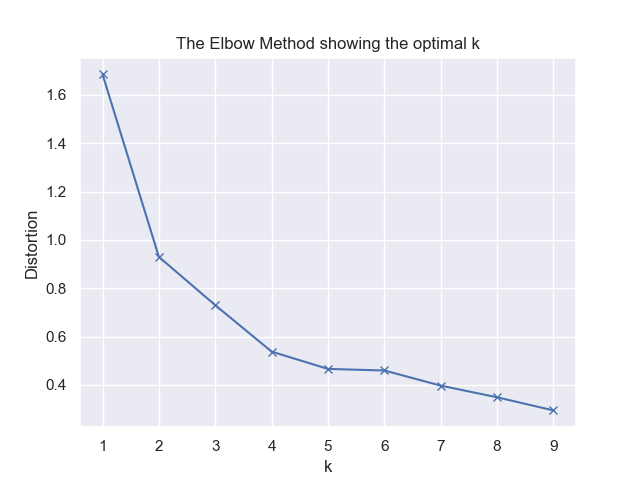
\includegraphics[width=0.8\linewidth]{Chapters/img/elbow_method.png}
\caption{Sum of squared error by number of clusters}
\label{fig:elbow_method}
\end{figure}



% section fishing_spots (end)



\section{SFA Library} % (fold)
\label{sub:sfa_library}

It was created a software application called SFALib for (Standalone Fishery Analysis Library. In this application, it was applied to the solutions described in this chapter to help with the elaboration and tests for this project. For a market solution, this library could be used by the main application of a Blue Box to send alerts to support decision making or to simply classify each VMS data entry as if fishing and if fishing in a new area for future analysis.



\subsection{Functionality} % (fold)
\label{sub:functionality}

This application allows to:
\begin{itemize}
\item Test new data \\ Send VMS data and receive it if it is considered to be fishing and if it is in a new area.
\item Test new velocity \\ Send sog data and receive true if it is considered to be fishing.
\item Test new location \\ Send GPS data and receive true it is in a new area.
\item Restart models \\ Request to create new models. It can be used if the objective is running for a long time and want to renew models with new data. 
\item Get limits \\ Request the velocity limits. Receive a tuple with two doubles (item1 = low-speed limit, item2 = high-speed limit). It can be used for analysis like is described in Chapter 5.
\end{itemize}

To make this possible is necessary to configure the data access layer to get the VMS data from the local data repository.
Correnlty, the application supports conection to SQL Server \cite{WEBSITE:SqlServer} and PostgreSQL \cite{WEBSITE:Postgresql}.


% subsection functionality (end)


\subsection{Architecture and Implementation} % (fold)
\label{sub:architecturee_implementation}
To develop the software, it was decided to use Java 8 \cite{WEBSITE:OraJava8} because it is a powerful, full object-oriented, and cross-platform programming language. MONICAP uses Linux, so using a JRE (Java Runtime Environment) application is a good choice.
The architecture is depicted in Figure \ref{fig:SFALib_Prof}. In this architecture is possible to distinguish three main modules: One that is the core of the SFALib, create the modules and use them. Another one is WEKA \cite{WEBSITE:Weka} that creates the cluster modules for locations and kernel density for velocity. The last one is the data access layer that is responsible for getting the VMS data from the local repository so SFALib can create the modules.


\begin{figure}[h]
\centering
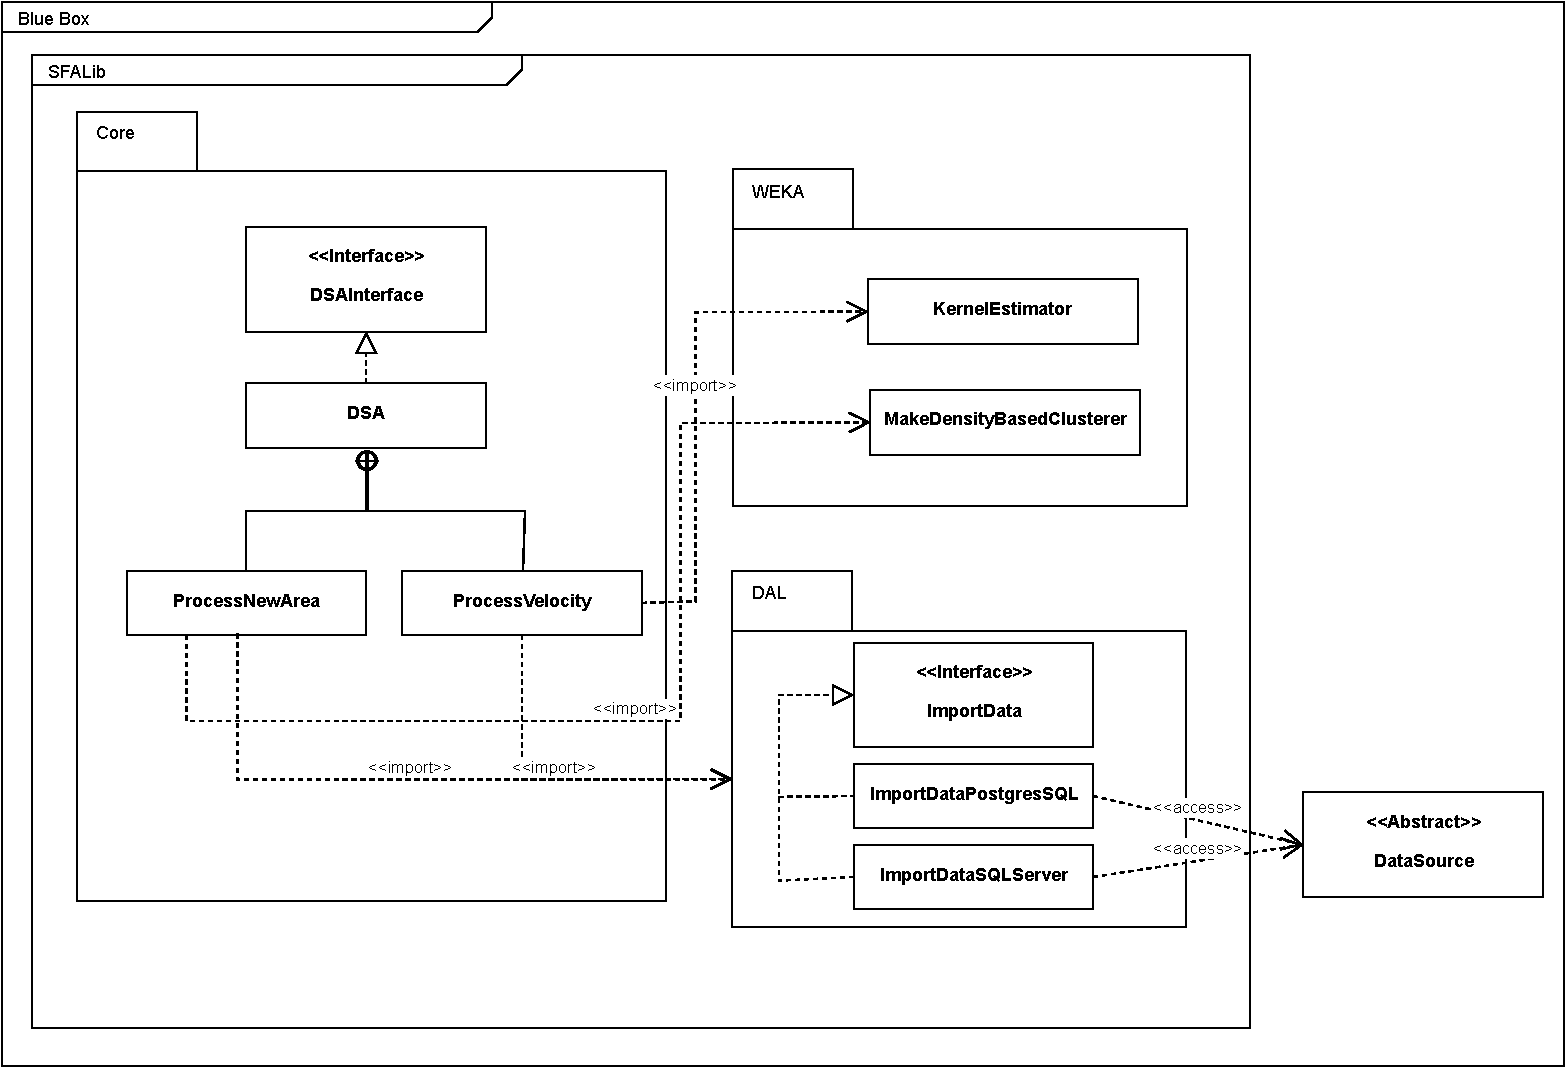
\includegraphics[width=1.0\linewidth]{Chapters/img/SFALib_Prof.pdf}
\caption{Representation of the SFALib architecture.}
\label{fig:SFALib_Prof}
\end{figure}



\textbf{Core module} \\The core module is responsible for initializing the models and using them the way described in this chapter. It starts by creating an instance of ProcessVelocity to create the first model and then create an instance of ProcessNewArea that uses the velocity limits previously obtained to get the locations data to form when the vessel was fishing to create the module.

\textbf{WEKA module} \\Weka is a collection of machine learning algorithms for data mining tasks. It contains tools for data preparation, classification, regression, clustering, association rules mining, and visualization. In this application, WEKA is used as a tool to create the modules.

\textbf{DAL module} \\The data access module was implemented in a way not only to get data but also to filter data in the database engine. Filtering data (where) is optimized on the database engine, and so we gain some performance.




The application starts by initializing two objects:
\begin{enumerate}
\item ProcessVelocity: This object is responsible for doing the process explained in point 4.2 of this document. This object will request to the static class ImportData to retrieve all SOG (Speed Over Ground) data from the database. Then the process will end with the limits (minimum speed of fishing and the maximal speed of fishing).
\item ProcessNewArea: This object is responsible for doing the process explained in point 4.3 of this document. This object is only initialized after ProcessVelocity because it needs the velocity fishing limits only to create the clusters of the fishing areas. With these limits, the object request to ImportData only the Lat and Lon where the vessel was in between the velocity limits. With this, the object ends up with the clusters of the fishing areas.
\end{enumerate}


% subsection architecturee_implementation (end)

\subsection{Deployment} % (fold)
\label{sub:deployment}

We start by initializing SFALib with the doubles limitVelocity and limitArea. This doubles range between 0 and 1:
\begin{itemize}
\item limitVelocity: used to get the maximum and minimum speed by reducing the speed range. This limit will reduce de maximum speed and increase the minimum speed by setting the maximum velocity as the velocity that as (1-limit) percentage of the cumulative kernel distribution and the minimum velocity as the velocity that as a (limit) percentage of the cumulative kernel distribution.
\item limitArea: used to compare with the probability to belong in a cluster given to the new points. If the limit is smaller than the given probability, then the vessel is classified as fishing in a new area.
\end{itemize}
These limits are important so we can configure if we prefer to have more false positive or false negative classifications.
A false positive (type I error) is when the classifier rejects a true hypothesis.
A false negative (type II error) is when the classifier accepts a false hypothesis.

After we have the SFALib ready we need to send a new velocity data and GPS coordinates to receive an object with an "isFishing" as true if the vessel is fishing and an "isNewArea" as true if the vessel is in an area that is not a normal fishing area and it's in a fishing velocity.

The methods that can be used are:
\begin{itemize}
\item newData method that receive VMS data and return isFishing(boolean) and isNewArea(boolean).
\item isFishing: method with SOG(double) as input and a boolean as output with, True = is fishing, False = not fishing.
\item isNewArea: method with GPS(double longitude, double latitude) as input and a boolean as output with, True = is fishing in a new area, False = not fishing in a new area.
\item restart: this method restart the models. It can be used to create models with new data.
\item GetLimit: the method used to get SOG limits used by the SFALib to classify velocity. As Limits(double min, double max) as output.
\end{itemize}
% subsection usage (end)

% section SFA_library (end)
% chapter blue_box (end)





